\documentclass{article}

\usepackage{graphicx}
\usepackage{tikz}
\usepackage{tikzsymbols}
\usetikzlibrary{calc,patterns,shapes.geometric}
\pagestyle{empty}
\usepackage[margin=0pt]{geometry}
\geometry{papersize={14in,12in}}

\def\centerarc[#1](#2)(#3:#4:#5){\draw[#1] ($(#2)+({#5*cos(#3)},{#5*sin(#3)})$) arc (#3:#4:#5);}

\begin{document}
	\begin{figure}
		\centering
		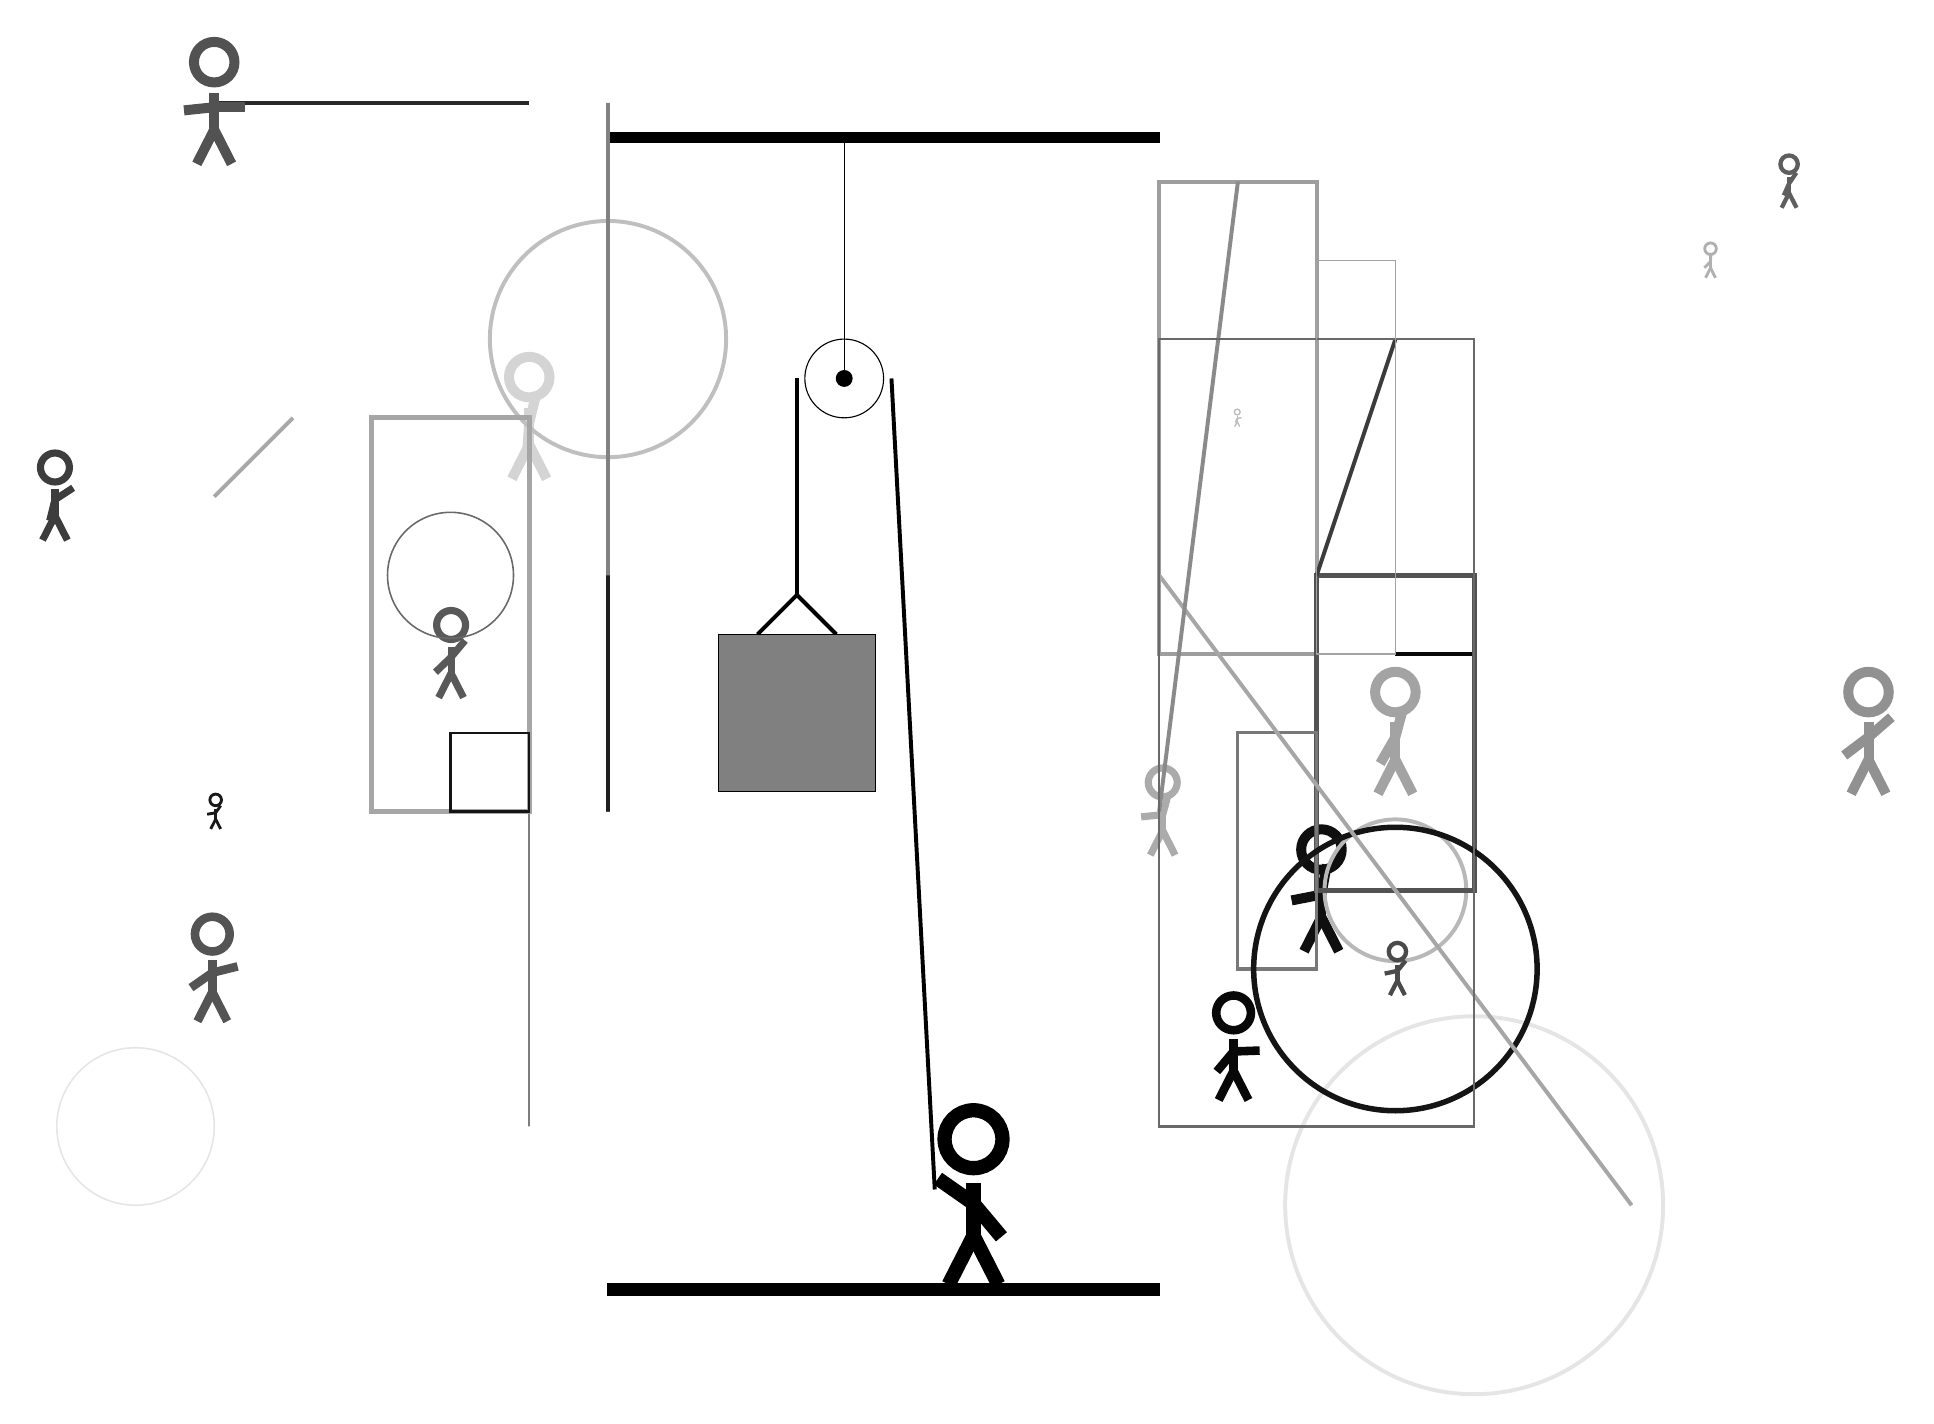
\begin{tikzpicture}
			%%%%% START %%%%%
			
			\draw[fill=black] (-2, 11.5) rectangle (5, 11.625);
			
			\node[line width=0.5mm, color=black!33] at (5, 3) {\Strichmaxerl[5][6][75]};
			
			\draw [line width=0.5mm, color=black!10](9, -2) circle (2.4);
			\node[line width=0.6mm, color=black!31] at (12, 10) {\Strichmaxerl[2][45][89]};
			\draw[line width=0.5mm, color=black!34](-7, 7) -- (-6, 8);
			\draw[line width=0.5mm, color=black!97](9, 5) -- (8, 5);
			
			\node[line width=0.5mm, color=black!26] at (6, 8) {\Strichmaxerl[1][64][10]};
			
			\node[line width=0.7mm, color=black!65] at (-4, 5) {\Strichmaxerl[5][44][50]};
			\node[line width=0.5mm, color=black!94] at (7, 2) {\Strichmaxerl[7][11][80]};
			\draw[line width=0.2mm, color=black!51] (-3, 6) rectangle (-3, -1);
			\node[line width=0.2mm, color=black!17] at (-3, 8) {\Strichmaxerl[7][86][76]};
			
			\draw [line width=0.5mm, color=black!28](8, 2) circle (0.9);
			\node[line width=0.3mm, color=black!90] at (-7, 3) {\Strichmaxerl[2][10][55]};
			\node[line width=0.2mm, color=black!36] at (8, 4) {\Strichmaxerl[7][60][75]};
			\node[line width=0.6mm, color=black!67] at (-7, 1) {\Strichmaxerl[6][35][14]};
			\draw [line width=0.5mm, color=black!25](-2, 9) circle (1.5);
			\draw[line width=0.6mm, color=black!35] (-3, 8) rectangle (-5, 3);
			\draw[line width=0.5mm, color=black!49] (-2, 3) rectangle (-2, 12);
			
			\draw[line width=0.5mm, color=black!38] (7, 5) rectangle (5, 11);
			\node[line width=0.3mm, color=black!63] at (13, 11) {\Strichmaxerl[3][66][56]};
			
			\draw [line width=0.2mm, color=black!59](-4, 6) circle (0.8);
			\draw[line width=0.6mm, color=black!68] (7, 2) rectangle (9, 6);
			
			\node[line width=0.7mm, color=black!97] at (6, 0) {\Strichmaxerl[6][50][2]};
			
			\draw[line width=0.4mm, color=black!53] (7, 4) rectangle (6, 1);
			\draw [line width=0.7mm, color=black!92](8, 1) circle (1.8);
			\node[line width=0.5mm, color=black!76] at (-9, 7) {\Strichmaxerl[5][76][33]};
			
			\draw[line width=0.3mm, color=black!92] (-4, 4) rectangle (-3, 3);
			
			\draw[line width=0.5mm, color=black!35](5, 6) -- (11, -2);
			\draw [line width=0.4mm, color=black!35](-6, 0) circle (0.0);
			
			\draw[line width=0.5mm, color=black!84](-7, 12) -- (-3, 12);
			\node[line width=0.4mm, color=black!71] at (8, 1) {\Strichmaxerl[3][12][51]};
			\draw[line width=0.5mm, color=black!46](5, 3) -- (6, 11);
			\draw[line width=0.5mm, color=black!77](8, 9) -- (7, 6);
			\node[line width=0.6mm, color=black!68] at (-7, 12) {\Strichmaxerl[7][6][0]};
			\draw[line width=0.6mm, color=black!88] (-2, 6) rectangle (-2, 3);
			\draw [line width=0.2mm, color=black!10](-8, -1) circle (1.0);
			\node[line width=0.6mm, color=black!43] at (14, 4) {\Strichmaxerl[7][37][41]};
			\draw[line width=0.3mm, color=black!59] (5, 9) rectangle (9, -1);
			
			\draw[line width=0.2mm, color=black!36] (7, 5) rectangle (8, 10);
			
			\draw (1, 8.5) circle (0.5);
			\draw[fill=black] (1, 8.5) circle (0.1);
			\draw (1, 11.5) -- (1, 8.5);
			
			\draw[line width=0.5mm] (-0.1, 5.25) -- (0.4, 5.75) -- (0.9, 5.25);
			\draw[fill=black!50] (-0.6, 5.25) rectangle (1.4, 3.25);
			
			\draw[line width=0.5mm] (0.4, 8.5) -- (0.4, 5.75);
			\centerarc[line width=0.5mm](1, 8.5)(0:180:0.6);
			\draw[line width=0.5mm](1.6, 8.5) -- (2.15, -1.8);
			
			\node at (2.6, -1.9) {\Strichmaxerl[10][-35][-50]};
			
			\draw[fill=black] (-2, -3) rectangle (5, -3.15);
			
			%%%%% END %%%%%
		\end{tikzpicture}
	\end{figure}	
\end{document}